\subsection{Scenari}
	\subsubsection{Gestione richiesta di registrazione}
	Il seguente diagramma rappresenta lo scenario con il quale viene gestita una richiesta di registrazione. La richiesta parte da signupService() e viene gestita da \textit{AuthController} che controlla il corretto inserimento dei dati e invia il responso a \textit{AuthController}, tramite postRegister(). Viene poi ritornata create() che indica a signupService che l'utente è stato creato.
	\begin{figure}[H]
		\centering
		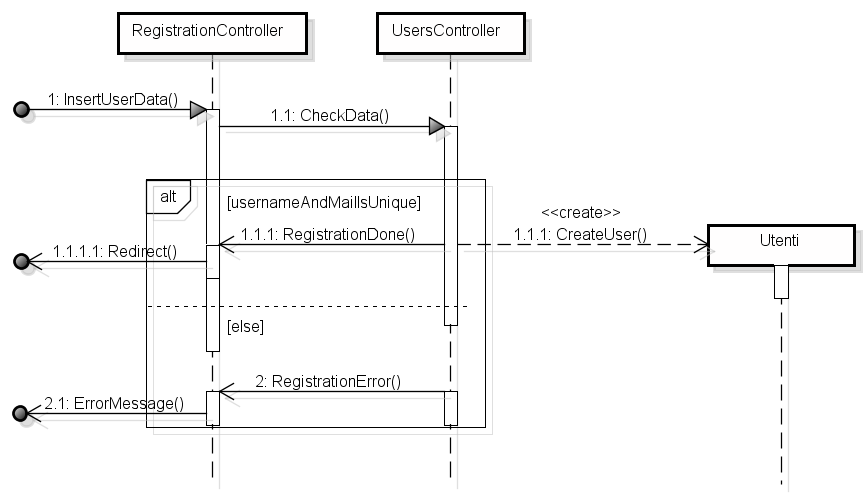
\includegraphics[scale=0.5]{img/register.png}
		\caption{Diagrammi di sequenza - Richiesta di registrazione}
	\end{figure}

\newpage
	\subsubsection{Gestione richiesta di autenticazione}
	Il loginService() invia una richiesta che viene gestita da \textit{AuthController}, il quale invia una postLogin() a \textit{AuthenticatesUsers}. Qui li scenari possibili sono due: nel primo caso la procedura va a buon fine e \textit{AuthenticatesUsers} emette un response() verso \textit{AuthController} che segnala a loginService() tramite una redirect() che l'autenticazione ha avuto successo. Nel secondo caso \textit{AuthenticatesUsers} invia una getFailedLoginMessage() a \textit{AuthController} che segnala l'errore a loginService() tramite un failed();

	\begin{figure}[H]
		\centering
		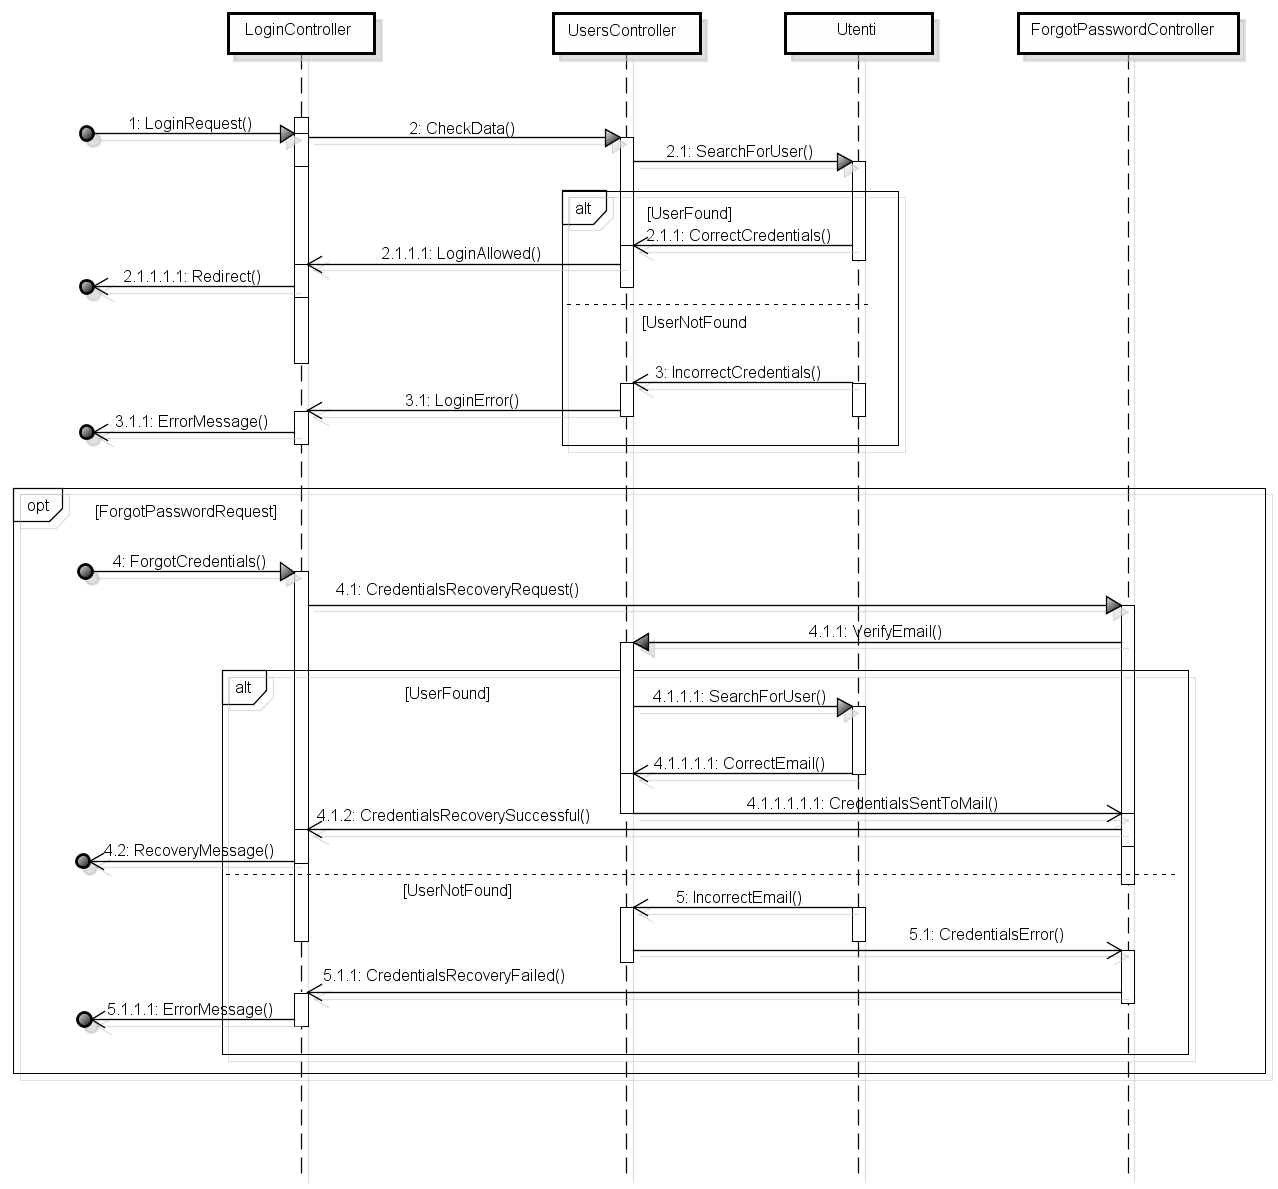
\includegraphics[width=0.9\textwidth]{img/login.png}
		\caption{Diagrammi di sequenza - Richiesta di autenticazione}
	\end{figure}

\newpage
	\subsubsection{Gestione richiesta di ricerca di un progetto}
	Una richiesta di ricerca inoltrata da searchService() viene gestita da \textit{SearchCtrl} che invia una search() a \textit{SearchController}. A questo punto viene ritornato un showResults a \textit{SearchCrtl} che a sua volta segnala i risultati ottenuti a searchService() con un sendResults().
	\begin{figure}[H]
		\centering
		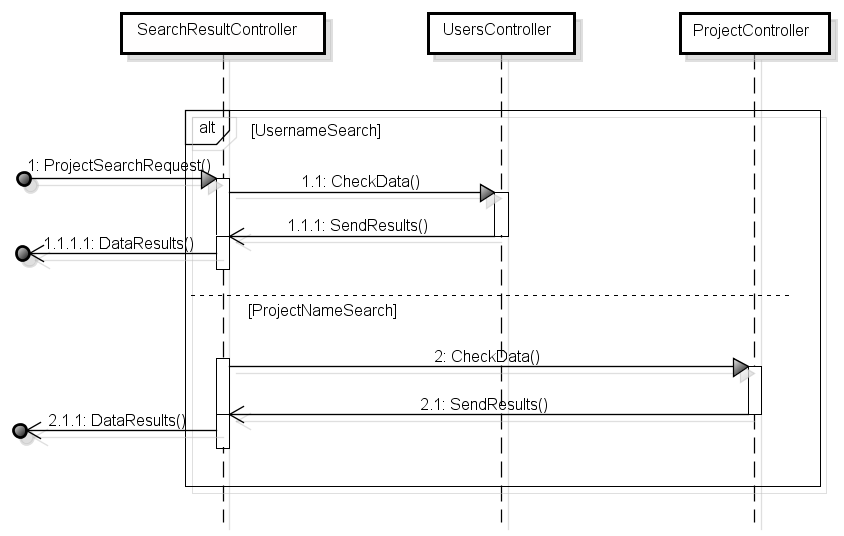
\includegraphics[scale=0.5]{img/search.png}
		\caption{Diagrammi di sequenza - Richiesta di ricerca di un progetto}
	\end{figure}
	
\newpage	
	\subsubsection{Gestione richiesta di visualizzazione di una presentazione}
	presentationService() invia una richiesta gestita da \textit{PresentationCtrl}. Esso invia una loadSlides() a \textit{PresentationController} il quale elabora le informazioni e emette una show() indirizzata a \textit{PresentationCtrl}. Questo controller alla fine invia il risultato di ritorno a presentationService() tramite il metodo slide in (slidesSVG).
	
	\begin{figure}[H]
		\centering
		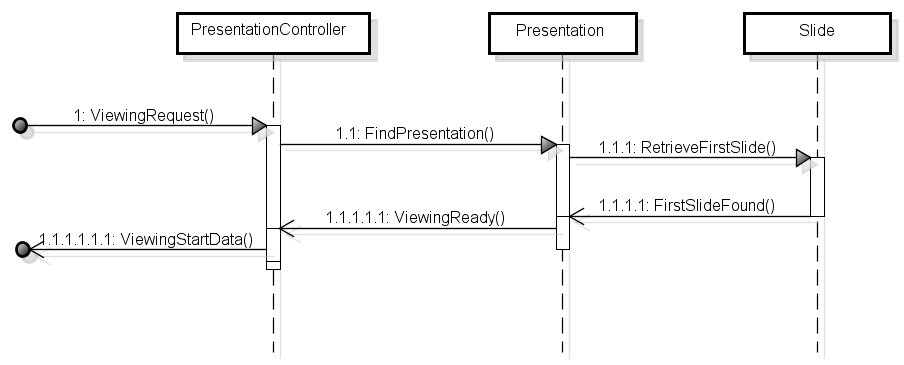
\includegraphics[scale=0.5]{img/view.png}
		\caption{Diagrammi di sequenza - Richiesta di visualizzazione di una presentazione}
	\end{figure} 
	
	
	\subsubsection{Gestione richiesta di creazione di un progetto}
	presentationEditorService() invia una richiesta che viene presa in carico dal \textit{PresentationCtrl}, che invia una createPresentation() a \textit{PresentationController}. Quest'ultimo elabora i dati ricevuti ed invia una show() a \textit{PresentationCtrl} che restituisce il risultato a presentationService() tramite il metodo slide in (slidesSVG).
	
	\begin{figure}[H]
		\centering
		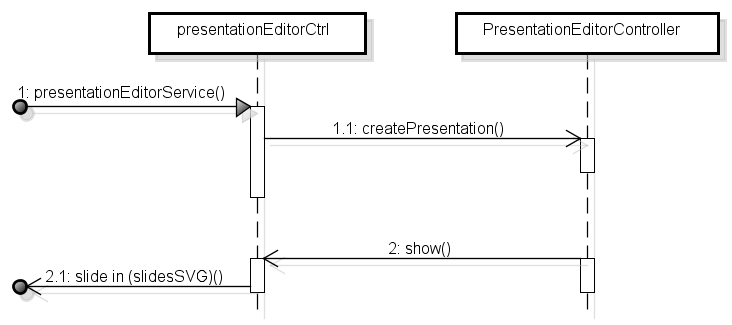
\includegraphics[scale=0.5]{img/create.png}
		\caption{Diagrammi di sequenza - Richiesta di creazione di un progetto}
	\end{figure}
	
\newpage	
	\subsubsection{Gestione richiesta di apertura di un progetto}
	Viene inviata una richiesta di apertura di un progetto da parte di openProjectService() e gestita da \textit{myProjectCtrl}. Questo invia una openProject() a \textit{Project} il quale invia load() gestita sempre da \textit{myProject}. Infine a openProjectService() viene passato il risultato delle operazioni effettuate tramite showProjectService().
	
	\begin{figure}[H]
		\centering
		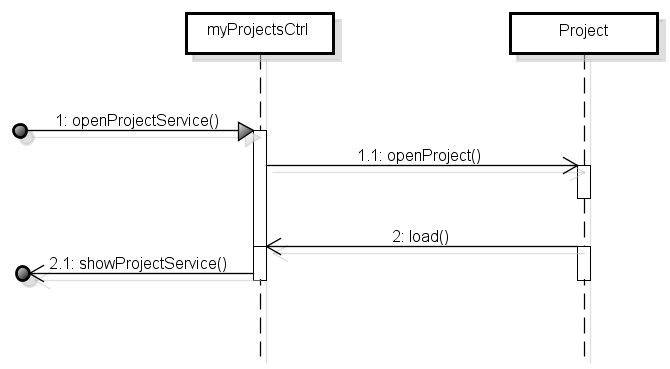
\includegraphics[scale=0.5]{img/open.png}
		\caption{Diagrammi di sequenza - Richiesta di apertura di un progetto}
	\end{figure}
	
	\newpage
	
	\subsubsection{Gestione richiesta di modifica di un progetto}
	slideEditorService() invia una richiesta gestita da \textit{SlideEditorCtrl}, che invia a sua volta un slideEditor() gestito da \textit{SlideController}. Esso invia una showEditor() a \textit{SlideEditorCtrl} che risponde con slideEditorShowService() alla chiamata iniziale.
	
	\begin{figure}[H]
		\centering
		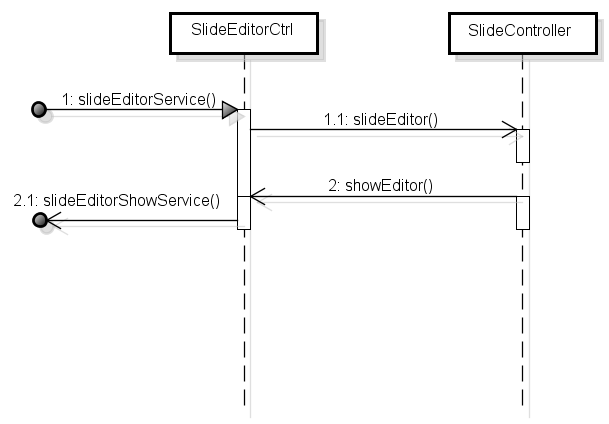
\includegraphics[scale=0.5]{img/modify.png}
		\caption{Diagrammi di sequenza - Richiesta di modifica di un progetto}
	\end{figure}
	
	
	
	\subsubsection{Gestione richiesta salvataggio di un progetto}
	saveProjectService() invia una richiesta che viene gestita da \textit{myProjectCtrl}, questo invia una saveProject() a \textit{ProjectController} che elabora i dati ed emette una store(). store() viene gestita da \textit{myProjectCtrl} che risponde alla chiamata iniziale tramite saveProjectService().
	
	\begin{figure}[H]
		\centering
		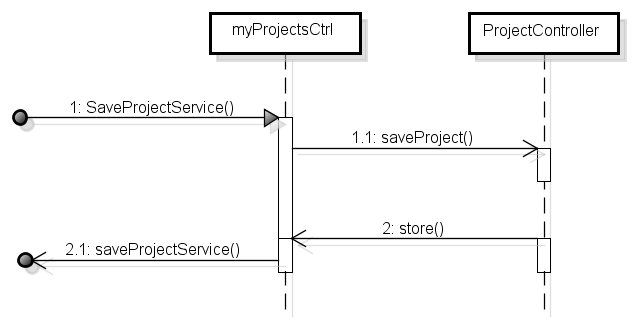
\includegraphics[scale=0.5]{img/save.png}
		\caption{Diagrammi di sequenza - Richiesta di salvataggio di un progetto}
	\end{figure}
	\newpage
